\documentclass{article}
\usepackage[left=3cm,top=3cm,right=2cm,bottom=2cm]{geometry}
\usepackage{amssymb}
\usepackage{amsmath}
\usepackage{cancel}
\usepackage{xcolor}
\usepackage{enumitem}
\usepackage{graphicx}
\usepackage[hidelinks]{hyperref}

\title{(Universidade de São Paulo)\\
Trabalho 01 - Temperaturas no Grafo de Manhattan}

\author{Métodos do Cálculo Numérico I -- SME0205\\
Docente: Antonio Castelo Filho\\[.2cm]
Julia Guazzelli Monteiro -- 15465383\\
Vinícius de Sá Ferreira -- 15491650}

\date{26 abr. 2025}

\begin{document}
    \maketitle
    
    \section{Modelagem do problema}

    Suponha $T: \mathbb{N} \times (\mathbb{R} \setminus \mathbb{R}^-) \to \mathbb{R}$ definida por $T(x,t) =$ \verb|temperatura no ponto |$x$\verb| ao tempo |$t$. Temos a equação do calor em 1D da seguinte forma
    \[\frac{\partial T(x,t)}{\partial t} = \alpha \frac{\partial^2 T(x,t)}{\partial x^2}\]
    onde $\alpha > 0$ é a difusão térmica. Assim podemos fazer a aproximação por série de Taylor para um $t_0$ fixo, ao redor de $x$
    \[T(x+1) = \sum_{j=0}^{+\infty} \frac{T^{(j)}(x) (\cancel{x}+1-\cancel{x})^j}{j!} = \sum_{j=0}^{+\infty} \frac{T^{(j)}(x)}{j!} = T(x) + T'(x) + \frac{T''(x)}{2} + \frac{T^{(3)}(x)}{6} + \frac{T^{(4)}(x)}{24} + \cdots\]
    \[T(x-1) = \sum_{j=0}^{+\infty} \frac{T^{(j)}(x) (\cancel{x}-1-\cancel{x})^j}{j!} = \sum_{j=0}^{+\infty} (-1)^j\frac{T^{(j)}(x)}{j!} = T(x) - T'(x) + \frac{T''(x)}{2} - \frac{T^{(3)}(x)}{6} + \frac{T^{(4)}(x)}{24} - \cdots\]
    \[T(x+1)+T(x-1) = 2T(x) + T''(x) + \frac{T^{(4)}(x)}{12} + \cdots\]
    \[ T''(x) = T(x+1)-2T(x)+T(x-1) - \frac{T^{(4)}(x)}{12} - \cdots\]
    \[\therefore T''(x) = T(x+1)-2T(x)+T(x-1) \color{gray}{- \mathcal{O}(1)}\]
    logo se definirmos $T_i(t) := T(t,i)$, teremos
    \[\frac{dT_i(t)}{dt} = \alpha (T_{i+1}(t)-2T_i(t)+T_{i-1}(t))\]

    Portanto, se tivermos $T(t) = \left[ \begin{array}{c}
        T_1(t)\\
        T_2(t)\\
        T_3(t)\\
        \vdots\\
        T_n(t)
    \end{array} \right]$, podemos reescrever a equação em função do Laplaciano $L$ do grafo, dado por $L = G-A$, com $G$ a matriz diagonal com o grau de arestas para cada vértice e $A$ a matriz de adjacência. Note que
    \[LT = \left( \left[ \begin{array}{ccccc}
        G_1 & 0 & 0 & \cdots & 0\\
        0 & G_2 & 0 & \cdots & 0\\
        0 & 0 & G_3 & \cdots & 0\\
        \vdots & \vdots & \vdots & \ddots & \vdots\\
        0 & 0 & 0 & \cdots & G_n
    \end{array} \right] - \left[ \begin{array}{ccccc}
        &&&&\\
        &&&&\\[.19cm]
        &&A&&\\
        &&&&\\[.19cm]
        &&&&\\
    \end{array} \right] \right)_{n \times n}\left[ \begin{array}{c}
        T_1\\
        T_2\\
        T_3\\
        \vdots\\
        T_n
    \end{array} \right]_{n \times 1} = \left[ \begin{array}{c}
        C_1\\
        C_2\\
        C_3\\
        \vdots\\
        C_n
    \end{array} \right]_{n \times 1}\]
    em que, para $i=1,2,3,\cdots,n$ teremos
    \[C_i = G_i T_i - \sum_{j \to i} T_j\]
    onde $j \to i$ indica os vizinhos de $i$, aqueles que estão conectados com $i$. No caso 1D, o grau de um ponto $i$ interno é de 2 e possui 2 pontos conexos, o sucessor e o antecessor, logo teremos a equação
    \[\frac{dT_i(t)}{dt} = \alpha (T_{i+1}(t)-2T_i(t)+T_{i-1}(t)) = -\alpha (2T_i(t) - T_{i-1}(t) - T_{i+1}(t)) = -\alpha (G_i T_i(t) - \sum_{j \to i} T_{j}(t)) = -\alpha (LT)_i\]

    Portanto, temos
    \[\frac{dT}{dt} = -\alpha LT\ (*)\]
    
    Uma forma de estender $T(t)$ para $\mathbb{R}$ é com $T(t) = e^{(-\alpha Lt)}T(0)$, onde $T(0) = T_0$. Assim
    \[\frac{dT}{dt} = \frac{d}{dt}[e^{(-\alpha Lt)}T(0)] = -\alpha L e^{(-\alpha Lt)}T(0) = -\alpha L (e^{(-\alpha Lt)}T(0)) = -\alpha L T(t)\]
    que satisfaz $(*)$. Por fim, se fizermos $\displaystyle{ \lim_{t \to +\infty} T(t) = T_\infty = \left[ \begin{array}{c}
        c_1\\
        c_2\\
        c_3\\
        \vdots\\
        c_n
    \end{array} \right] }$, $c_i \in \mathbb{R}$, logo $\dfrac{dT}{dt} = \vec 0$ e a equação fica da seguinte forma
    \[\frac{dT}{dt} = -\alpha LT_\infty = \vec{0}\]
    \[LT_\infty = \vec{0}\]
    \[T_{i+1}(t)-2T_i(t)+T_{i-1}(t) = 0\]
    \[\therefore T_i(t) = \frac{T_{i-1}(t)+T_{i+1}(t)}{2}\]

    Agora, podemos adicionar condições de contorno, então teremos para $b$ o vetor com a temperatura em alguns pontos 
    \[\frac{dT}{dt} = -\alpha LT + b = 0\]
    \[\alpha LT = b\]

    Com a matriz de penalidades, ajustamos a contribuição resultando em

    \[(L+P)T = Pb\]

    \newpage

    \section{Métodos diretos}

    \subsection{Método de Cholesky}

    Suponhamos que $M$ seja uma matriz triangular simples, mais precisamente, uma matriz pequena, triangular e bem-comportada, então, pela teoria, achar na $M^{-1}$ explicitamente não seria algo muito complexo. Exemplo:

    \[
    \begin{bmatrix}
    2 & 1 & 3 \\
    0 & 1 & 2 \\
    0 & 0 & 4
    \end{bmatrix}
    \]

    Acharemos $U^{-1}$ usando $[U|I] \rightarrow [I|U^{-1}]$:

    \[
    [U|I] = 
    \begin{bmatrix}
    2 & 1 & 3 & \vline & 1 & 0 & 0 \\
    0 & 1 & 2 & \vline & 0 & 1 & 0 \\
    0 & 0 & 4 & \vline & 0 & 0 & 1
    \end{bmatrix}
    \rightarrow
    \begin{bmatrix}
    1 & 1/2 & 3/2 & \vline &  1/2 & 0 & 0 \\
    0 & 1 & 2 & \vline & 0 &  1 & 0 \\
    0 & 0 & 1 & \vline & 0 &  0 & 1/4
    \end{bmatrix}
    \]

    \[
    \begin{bmatrix}
    1 & 1/2 & 0 & \vline & 1/2 & 0 & -3/8 \\
    0 & 1 & 0 & \vline & 0 & 1 & -1/2 \\
    0 & 0 & 1 & \vline & 0 & 0 & 1/4
    \end{bmatrix}
    \rightarrow
    \begin{bmatrix}
    1 & 0 & 0 & \vline & 1/2 & -1/2 & -1/8 \\
    0 & 1 & 0 & \vline & 0 & 1 & -1/2 \\
    0 & 0 & 1 & \vline & 0 & 0 & 1/4
    \end{bmatrix}
    \]

    \[
    U^{-1} =
    \begin{bmatrix}
    1/2 & -1/2 & -1/8 \\
    0 & 1 & -1/2 \\
    0 & 0 & 1/4
    \end{bmatrix}
    \]

    Mas se tivermos uma matriz geral (não necessariamente triangular), mas invertível, de entradas significativamente grandes (com linhas, colunas na casa dos milhares), então o número de operações para computar a inversa explicitamente pelo algoritmo de Gauss-Jordan (demonstrado de forma simplificada no exemplo acima com a matriz triangular) cresceria cubicamente com o tamanho $N$ da matriz, ou seja, seria $O(N^3)$ no que tange à análise assintótica. Pois, em termos simples, há $O(N)$ passos principais (um para cada coluna/pivô) na eliminação, e em cada passo, se opera em $O(N)$ linhas abaixo/acima do pivô, afetando $O(N)$ elementos em cada linha - as colunas à direita. A complexidade vem de algo como $O(N \text{ passos}) * O(N \text{ linhas afetadas}) * O(N \text{ operações por elemento}) = O(N^3)$. Para o computador, calcular a inversa explicitamente é, portanto, custoso. Para o humano, bem, deixaremos a discussão de lado.

    Para contra-atacar o alto custo da complexidade computacional na resolução do sistema $M x = k$, assumindo que a matriz seja simétrica e def. positiva, podemos pensar em fatorizar a matriz em questão em $M = LL^T$, onde $L$ é uma matriz triangular inferior (e $L^T$ é triangular superior). A própria fatorização de Cholesky tem um custo da ordem de $O(N^3)$ (embora geralmente com uma constante menor que a da inversão). Mas a vantagem crucial vem a seguir: em vez de calcular $M^{-1}$, resolvemos o sistema original $(LL^T)x = k$ em duas etapas, introduzindo $y = L^T x$:

    \begin{enumerate}
        \item Resolver $Ly = k$ para $y$ usando substituição \textbf{direta}.
        \item Resolver $L^T x = y$ para $x$ usando substituição \textbf{retroativa}.
    \end{enumerate}

    Cada uma dessas etapas de substituição tem um custo muito menor, da ordem de $O(N^2)$. Portanto, após o custo inicial da fatorização ($O(N^3)$), a solução do sistema em si é muito menos complexa ($O(N^2)$) do que calcular a inversa completa ($O(N^3)$) e depois multiplicar por $k$ ($O(N^2)$). É nisso que o algoritmo de Cholesky se baseia para ser eficiente na resolução de sistemas lineares.

    \subsubsection{Conexão com o código}

    A fatoração da decomposição da matriz $M$ no produto de uma matriz triangular inferior $L$ e sua transposta $L^T$ é realizada pela função abaixo no código.

    \begin{center}
    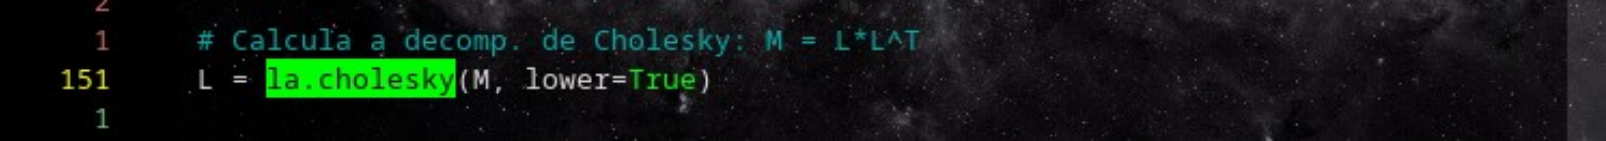
\includegraphics[width=0.8\linewidth]{imgs/cholesky_1.png}
    \end{center}

    Depois de obter $L$, a solução é encontrada resolvendo dois sistemas triangulares sequencialmente e retornando o vetor $x$:

    \begin{center}
    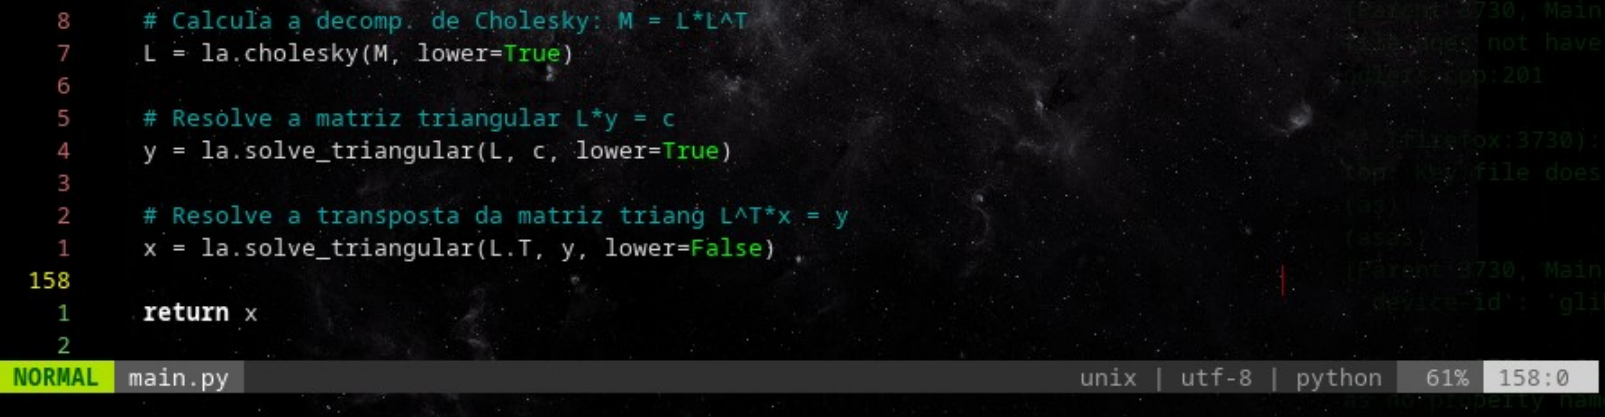
\includegraphics[width=0.8\linewidth]{imgs/cholesky_2.png}
    \end{center}

    Embora a etapa de fatoração ainda domine a complexidade ($O(N^3)$), a constante multiplicativa é menor do que em métodos como LU ou QR para matrizes densas, o cálculo de comparação do tempo de execução será discutido mais posteriormente.

    \subsection{Método LU}

    Fazendo uma breve comparação com o método de Cholesky, o algoritmo LU não requer que a matriz $M$ seja simétrica ou definida positiva, basta que ela seja quadrada e invertível - isso generaliza as aplicações de uma forma significativa.

    Porém mesmo para matrizes quadradas e invertíveis com entradas muito grandes, calcular a inversa $M^{-1}$ diretamente (explicitamente) ou usar métodos muito básicos tende a ser computacionalmente caro (complexidade $O(N^3)$) e propenso a erros numéricos.

    A saída seria usar a decomposição LU que se consiste em fatorar a matriz $M$ de forma a simplificar a resolução do sistema. E para evitar divisões por zero ou números muito pequenos, o processo pode incluir pivotamento, que troca as linhas da matriz durante a fatoração. Em suma, isso resulta na decomposição:
    \[ PM = LU \]
    onde:

    \begin{itemize}[leftmargin=*]
        \item $P$ é uma matriz de permutação;
        \item $L$ é uma matriz triangular inferior;
        \item $U$ é uma matriz triangular superior.
    \end{itemize}

    \subsubsection{Resolução do Sistema com Decomposição LU}

    Com essa fatoração, o sistema $MT = c$ se torna $LUT = Pc$. Podemos resolver isso em duas etapas, envolvendo sistemas triangulares, que já sabemos que são mais fáceis e rápidos de resolver (complexidade $O(N^2)$ cada):

    \begin{enumerate}
        \item Resolver $Ly = Pc$ para achar um vetor intermediário $y$. (Note que aplicamos a permutação $P$ ao vetor $c$).
        \item Resolver $UT = y$ para achar a solução final $T$
    \end{enumerate}

    A etapa mais custosa ainda é a fatoração $PM = LU$, que tem complexidade $O(N^3)$ (aproximadamente $\dfrac{2}{3}N^3$ operações para matrizes densas). Em teoria, esse método tem a mesma ordem de complexidade de Cholesky, mas na prática LU geralmente requer mais operações por não explorar a simetria da matriz (quando presente).

    \subsubsection{Conexão com o código}

    Fatoração da matriz $PM$ no produto $LU$:

    \begin{center}
    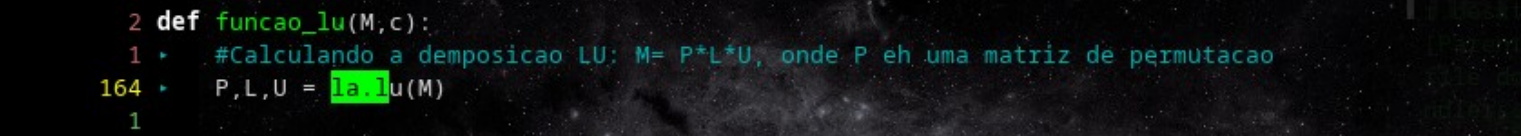
\includegraphics[width=0.8\linewidth]{imgs/lu_1.png}
    \end{center}

    Ao obter $P$, $L$, e $U$, encontramos $T$ resolvendo os dois sistemas triangulares sequencialmente, como implementado na função funcao\_lu:

    \begin{center}
    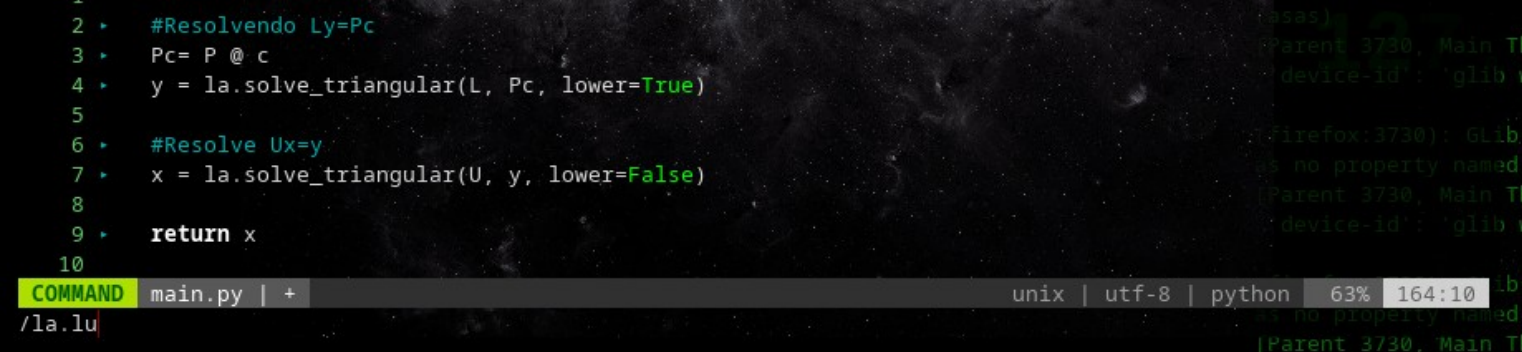
\includegraphics[width=0.8\linewidth]{imgs/lu_2.png}
    \end{center}

    \subsection{Método QR}

    De praxe, a decomposição QR é outro método fundamental para resolver sistemas lineares, porém com uma excelente estabilidade numérica, sendo particularmente robusto mesmo para matrizes mal-condicionadas. O método é aplicável a matrizes quadradas invertíveis gerais e não requer simetria ou definição positiva, também é a base para muitos algoritmos de autovalores e problemas de mínimos quadrados.

    A ideia central da decomposição QR é fatorar a matriz $M$ no produto de uma matriz ortogonal $Q$ e uma matriz triangular superior $R$:
    \[ M = QR \]
    onde:

    \begin{itemize}
        \item $Q$ é uma matriz ortogonal. Isso significa que suas colunas formam um conjunto ortonormal de vetores, e sua transposta é comutativa à sua inversa ($Q^TQ = QQ^T = I$, onde $I$ é a matriz identidade). Multiplicar por $Q$ ou $Q^T$ preserva normas e ângulos, o que contribui para a estabilidade numérica.
        
        \item $R$ é uma matriz triangular superior.
    \end{itemize}

    Com a fatoração $M = QR$, o sistema original $MT = c$ se torna $QRT = c$. Para isolar $T$, multiplicamos ambos os lados pela transposta (que é a inversa) de $Q$:

    \begin{align*}
    Q^T (QRT) &= Q^T c \\
    (Q^TQ)RT &= Q^T c \\
    I RT &= Q^T c \\
    RT &= Q^T c
    \end{align*}

    Isso resulta em um sistema triangular superior $RT = Q^T c$, que pode ser resolvido eficientemente por substituição retroativa (complexidade $O(N^2)$).

    A etapa computacionalmente mais intensiva é a própria fatoração $M = QR$. Existem diferentes algoritmos para computá-la (como Gram-Schmidt modificado, transformações de Householder ou rotações de Givens). Para matrizes densas, a complexidade da fatoração QR é geralmente $O(N^3)$, tipicamente com uma constante maior do que a da decomposição LU (aproximadamente $\frac{4}{3}N^3$ operações usando Householder). Portanto, embora seja muito estável, tende a ser mais custoso que LU ou Cholesky (quando aplicável) para a simples solução de sistemas lineares quadrados.

    \subsubsection{Conexão com o código}

    Fatoração da matriz $M$ no produto $QR$:

    \begin{center}
    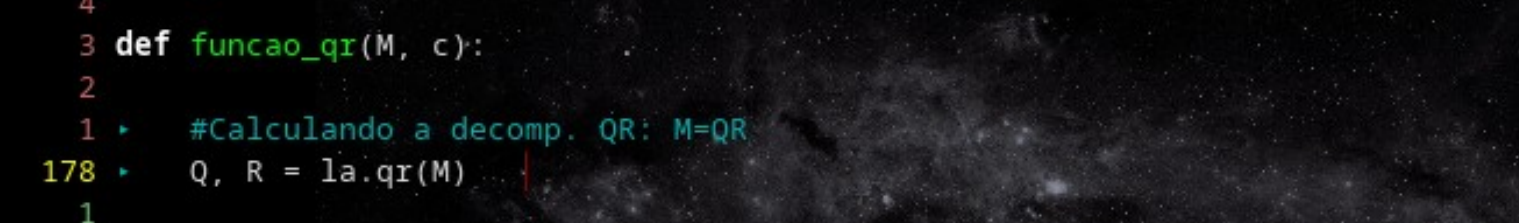
\includegraphics[width=0.8\linewidth]{imgs/qr_1.png}
    \end{center}

    Após obter $Q$ e $R$, a solução $T$ é encontrada calculando $Q^T c$ e depois resolvendo o sistema triangular $RT = Q^T c$, como implementado na função funcao\_qr:

    \begin{center}
    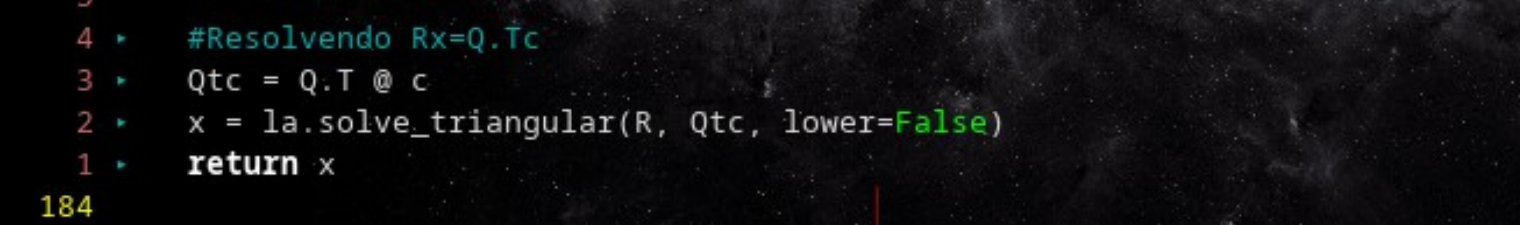
\includegraphics[width=0.8\linewidth]{imgs/qr_2.png}
    \end{center}

    \hypertarget{1}{}
    \hypertarget{5}{}

    \subsection{Resultados}

    Os tempos de execução registrados para cada método foram plotados no gráfico de barras, observada na \hyperlink{2}{\texttt{Figura 5}} para 9 pontos e na \hyperlink{6}{\texttt{Figura 12}}, para 435 pontos. Ao fazer a análise, observa-se que, para a matriz $M$ específica deste problema, que é simétrica e definida positiva (se trata de um grafo), o método de Cholesky apresentou o melhor desempenho, sendo o mais rápido entre as implementações baseadas em decomposição.

    Isso está de acordo com a teoria e o que foi estudado nas análises dos métodos que conduzimos, pois Cholesky explora a simetria da matriz, resultando em aproximadamente metade das operações de ponto flutuante em comparação com a decomposição LU para matrizes densas (aproximadamente $\dfrac{1}{3}N^3$ vs $\dfrac{2}{3}N^3$ operações para a fatoração). A função \texttt{numpy.linalg.solve}, sendo uma aplicação altamente otimizada (frequentemente baseada em implementações LAPACK), apresentou um desempenho muito competitivo, potencialmente detectando a natureza da matriz e utilizando um solver apropriado internamente.

    Além do mais, no que tange à análise minuciosa, a decomposição LU foi mais lenta que Cholesky, como esperado, por ser um método mais geral. A decomposição QR, embora robusta numericamente, tende a ser a mais custosa computacionalmente para a solução de sistemas lineares (com uma constante associada à complexidade $O(N^3)$ tipicamente maior, como $\dfrac{4}{3}N^3$ para métodos baseados em Householder), o que se refletiu em seu tempo de execução sendo o mais elevado entre os quatro métodos testados.

    Em suma, para o sistema linear derivado deste problema específico, a decomposição de Cholesky é a escolha mais eficiente em termos de tempo de execução, devido às propriedades favoráveis da matriz $M$. A função genérica \texttt{numpy.linalg.solve} também se mostrou extremamente eficaz. A escolha entre LU e QR dependeria de um balanço entre generalidade, custo computacional e requisitos de estabilidade numérica, sendo QR preferível em casos de matrizes mal-condicionadas, apesar de seu maior custo.

    \newpage

    \section{Métodos iterativos}

    \subsection{Gauss-Jacobi}
    Queremos resolver o sistema $Mx = c$, em que $M = (L+P)T$ e $c = Pb$. Assim, temos
    \[Mx = c\]
    \[(M-D+D)x = c\]
    \[(M-D)x + Dx = c\]
    \[(M-D)x^{(k)} + Dx^{(k+1)} = c\]
    \[Dx^{(k+1)} = (D-M)x^{(k)} + c\]
    \[x^{(k+1)} = D^{-1}(D-M)x^{(k)}+D^{-1}c\]
    \[x^{(k+1)} = (I-D^{-1}M)x^{(k)}+D^{-1}c\]
    \[x^{(k+1)} = Cx^{(k)} + g\]
    Como $D$ é a diagonal de $M$, o determinante é o produtório da diagonal e $M$ que é não-nulo, então $D$ é inversível.

    \subsection{Gauss-Seidel}
    Queremos resolver o sistema $Mx = c$, em que $M = (L+P)T$ e $c = Pb$. Assim, façamos $M = L+R$, onde $L$ é a matriz triangular inferior de $M$ e $R$, a triangular superior sem a diagonal, então
    \[Mx = c\]
    \[(L+R)x = c\]
    \[Lx + Rx = c\]
    \[Lx^{(k+1)} + Rx^{(k)} = c\]
    \[Lx^{(k+1)} = - Rx^{(k)} + c\]
    \[x^{(k+1)} = (-L^{-1}R)x^{(k)} + L^{-1}c\]
    \[x^{(k+1)} = Cx^{(k)} + g\]

    Como $L$ é triangular inferior, o determinante é o produtório da diagonal de $M$ que é não-nulo, então $L$ é inversível.

    \subsection{Gradientes conjugados}
    Queremos resolver o sistema $Mx = c$, em que $M = (L+P)T$ e $c = Pb$. Considere a função
    \[f(x) = \frac{1}{2}x^TMx - c^Tx\]
    onde $M$ é simétrica positiva definida (SPD). Note que
    \[f(x) = \frac{1}{2} \sum_{i=1}^{n}\sum_{j=1}^{n} m_{ij} x_{i} x_{j} - \sum_{i=1}^{n} c_{i} x_{i}\]
    \[\frac{\partial f(x)}{\partial x_k} = \frac{1}{2} \left( \sum_{i=1}^{n}\sum_{j=1}^{n} m_{ij} (x_{i} \delta_{ik} + x_{j} \delta_{jk}) \right) - c_k = \frac{1}{2} \left( \sum_{i=1}^{n} m_{ik} x_{i} + \sum_{j=1}^{n} m_{kj} x_{j} \right) - c_k\]
    \[= \frac{1}{\cancel{2}} \left( \cancel{2} \sum_{j=1}^{n} m_{kj} x_{j} \right) - c_k = \sum_{j=1}^{n} m_{kj} x_{j} - c_k\]
    \[\therefore \nabla f(x) = Mx - c\]

    \newpage

    Assim, queremos encontrar $x$ (que é único, porque $M$ é SPD) tal que $\nabla f(x) = 0 \iff Mx-c = 0 \iff Mx = c$.

    Começamos com um chute inicial $x_0$, então teremos um resíduo $r_0 = c - Mx_0 = -\nabla f(x_0)$. Teremos a direção inicial dada por $p_0 = r_0$, assim atualizamos
    \[x_1 = x_0 + \alpha p_0\]
    Temos que $r_1^T \cdot r_0 = 0$, porque são ortogonais, e $r_1 = c-Mx_1$, então
    \[r_1^T \cdot r_0 = 0\]
    \[(c-Mx_1)^T \cdot r_0 = 0\]
    \[[c-M(x_0 + \alpha p_0)]^T \cdot r_0 = 0\]
    \[(c-Mx_0)^T \cdot r_0 - \alpha(Mp_0)^T \cdot r_0 = 0\]
    \[(c-Mx_0)^T \cdot r_0 - \alpha(Mp_0)^T \cdot p_0 = 0\]
    \[(c-Mx_0)^T \cdot r_0 = \alpha(Mp_0)^T \cdot p_0\]
    \[\alpha = \frac{(c-Mx_0)^T \cdot r_0}{(Mp_0)^T \cdot p_0}\]
    \[\alpha = \frac{r_0^T \cdot r_0}{p_0^T \cdot M \cdot p_0}\]
    Agora fazemos $r_1 = r_0 - \alpha(Mp_0)$ e a direção deve ser atualizada de forma conjugada, isto é, $p_{k+1}^T \cdot M \cdot p_k = 0$. Então podemos fazer
    \[p_1 = r_1 + \beta p_0\]
    \[p_{1}^T \cdot M \cdot p_0 = 0\]
    \[(r_1 + \beta p_0)^T \cdot M \cdot p_0 = 0\]
    \[r_1^T \cdot M \cdot p_0 + \beta (p_0^T \cdot M \cdot p_0) = 0\]
    \[\beta (p_0^T \cdot M \cdot p_0) = -r_1^T \cdot M \cdot p_0\]
    \[\beta = -\frac{r_1^T \cdot M \cdot p_0}{p_0^T \cdot M \cdot p_0} = -\frac{r_1^T \cdot M \cdot p_0}{r_0^T \cdot M \cdot p_0}\]
    Como $r_1 = r_0 - \alpha(Mp_0)$, temos $\dfrac{1}{\alpha}(r_0 - r_1) = M \cdot p_0$, então
    \[\beta = -\frac{r_1^T \cdot \left[\cancel{\dfrac{1}{\alpha}}(r_0 - r_1)\right]}{r_0^T \cdot \left[\cancel{\dfrac{1}{\alpha}}(r_0 - r_1)\right]} = - \frac{\cancel{r_1^T \cdot r_0} - r_1^T \cdot r_1}{r_0^T \cdot r_0 - \cancel{r_0^T \cdot r_1}} = - \frac{- r_1^T \cdot r_1}{r_0^T \cdot r_0}\]
    \[\beta = \frac{r_1^T \cdot r_1}{r_0^T \cdot r_0}\]

    \newpage

    Portanto, as etapas são
    {\hspace{2cm}
    \begin{enumerate}[leftmargin=2cm]
        \item Chute inicial $x_0$;
        \item $p_0 = r_0 = c - Mx_0$;
        \item $\alpha = \dfrac{r_k^T \cdot r_k}{p_k^T \cdot M \cdot p_k}$;
        \item $x_{k+1} = x_k + \alpha p_k$;
        \item $r_{k+1} = r_k - \alpha (M \cdot p_k)$;
        \item $\beta = \dfrac{r_{k+1}^T \cdot r_{k+1}}{r_k^T \cdot r_k}$;
        \item $p_{k+1} = r_{k+1} + \beta p_k$;
        \item Volta para o passo 3, enquanto $\|r_{k+1}\| > $ tol.
    \end{enumerate}
    }

    \hypertarget{3}{}
    \hypertarget{7}{}

    \subsection{Resultados}

    \[\renewcommand{\arraystretch}{1.5}
    \begin{array}{|c|c|c|c|c|c|}
        \hline
        \text{Pontos} & \text{Tolerância} & & \text{Gauss-Jacobi} & \text{Gauss-Seidel} & \text{Gradientes Conjugados}\\
        \hline
        \smash{\raisebox{-.3cm}{9}} & \smash{\raisebox{-.3cm}{$10^{-1}$}} & k & 13000 & 7129 & 630\\
        \cline{3-6}
        & & \text{t} & 19\text{ min} & 11\text{ min} & 1\text{ min}\\
        \hline
        \smash{\raisebox{-.3cm}{435}} & \smash{\raisebox{-.3cm}{$10^{-3}$}} & k & 1261 & 647 & 251\\
        \cline{3-6}
        & & \text{t} & 3\text{ min} & 2\text{ min} & 30\text{ s}\\
        \hline
    \end{array}\]

    É possível observar os tempos exatos de execução na \hyperlink{4}{\texttt{Figura 6}} para 9 pontos e na figura \hyperlink{8}{\texttt{Figura 12}}, para 435 pontos.

    \section{Resultado obtido}

    \begin{figure}[ht]
        \centering
        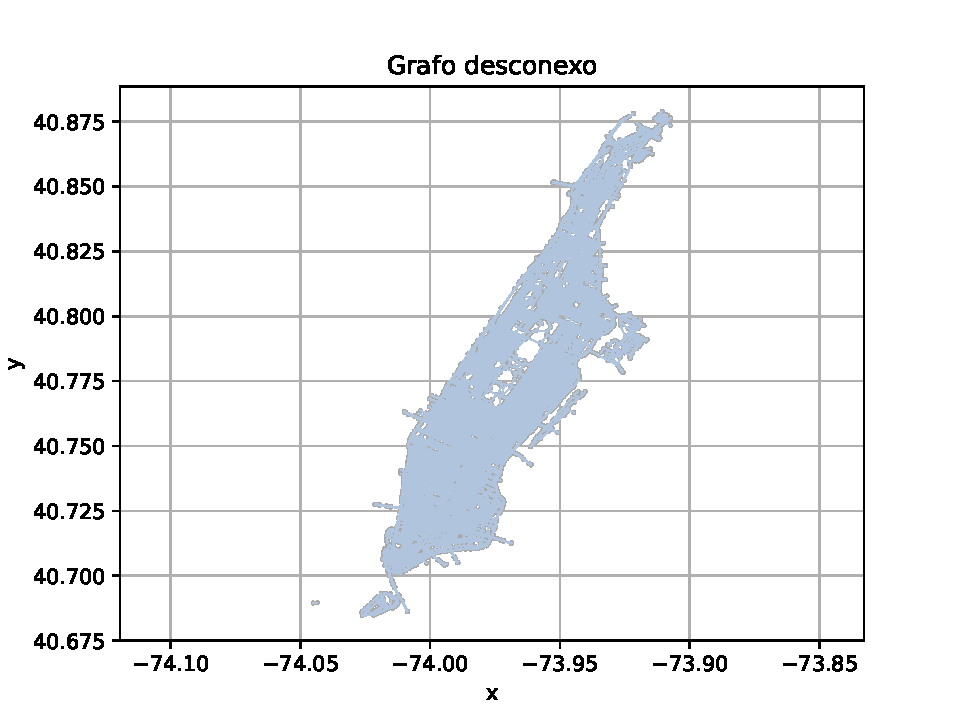
\includegraphics[width=0.6\textwidth, trim={0 .3cm 0 .9cm},clip]{../figs/fig1.pdf}
        
        Figura 1
    \end{figure}

    \newpage

    \begin{figure}[ht]
        \centering
        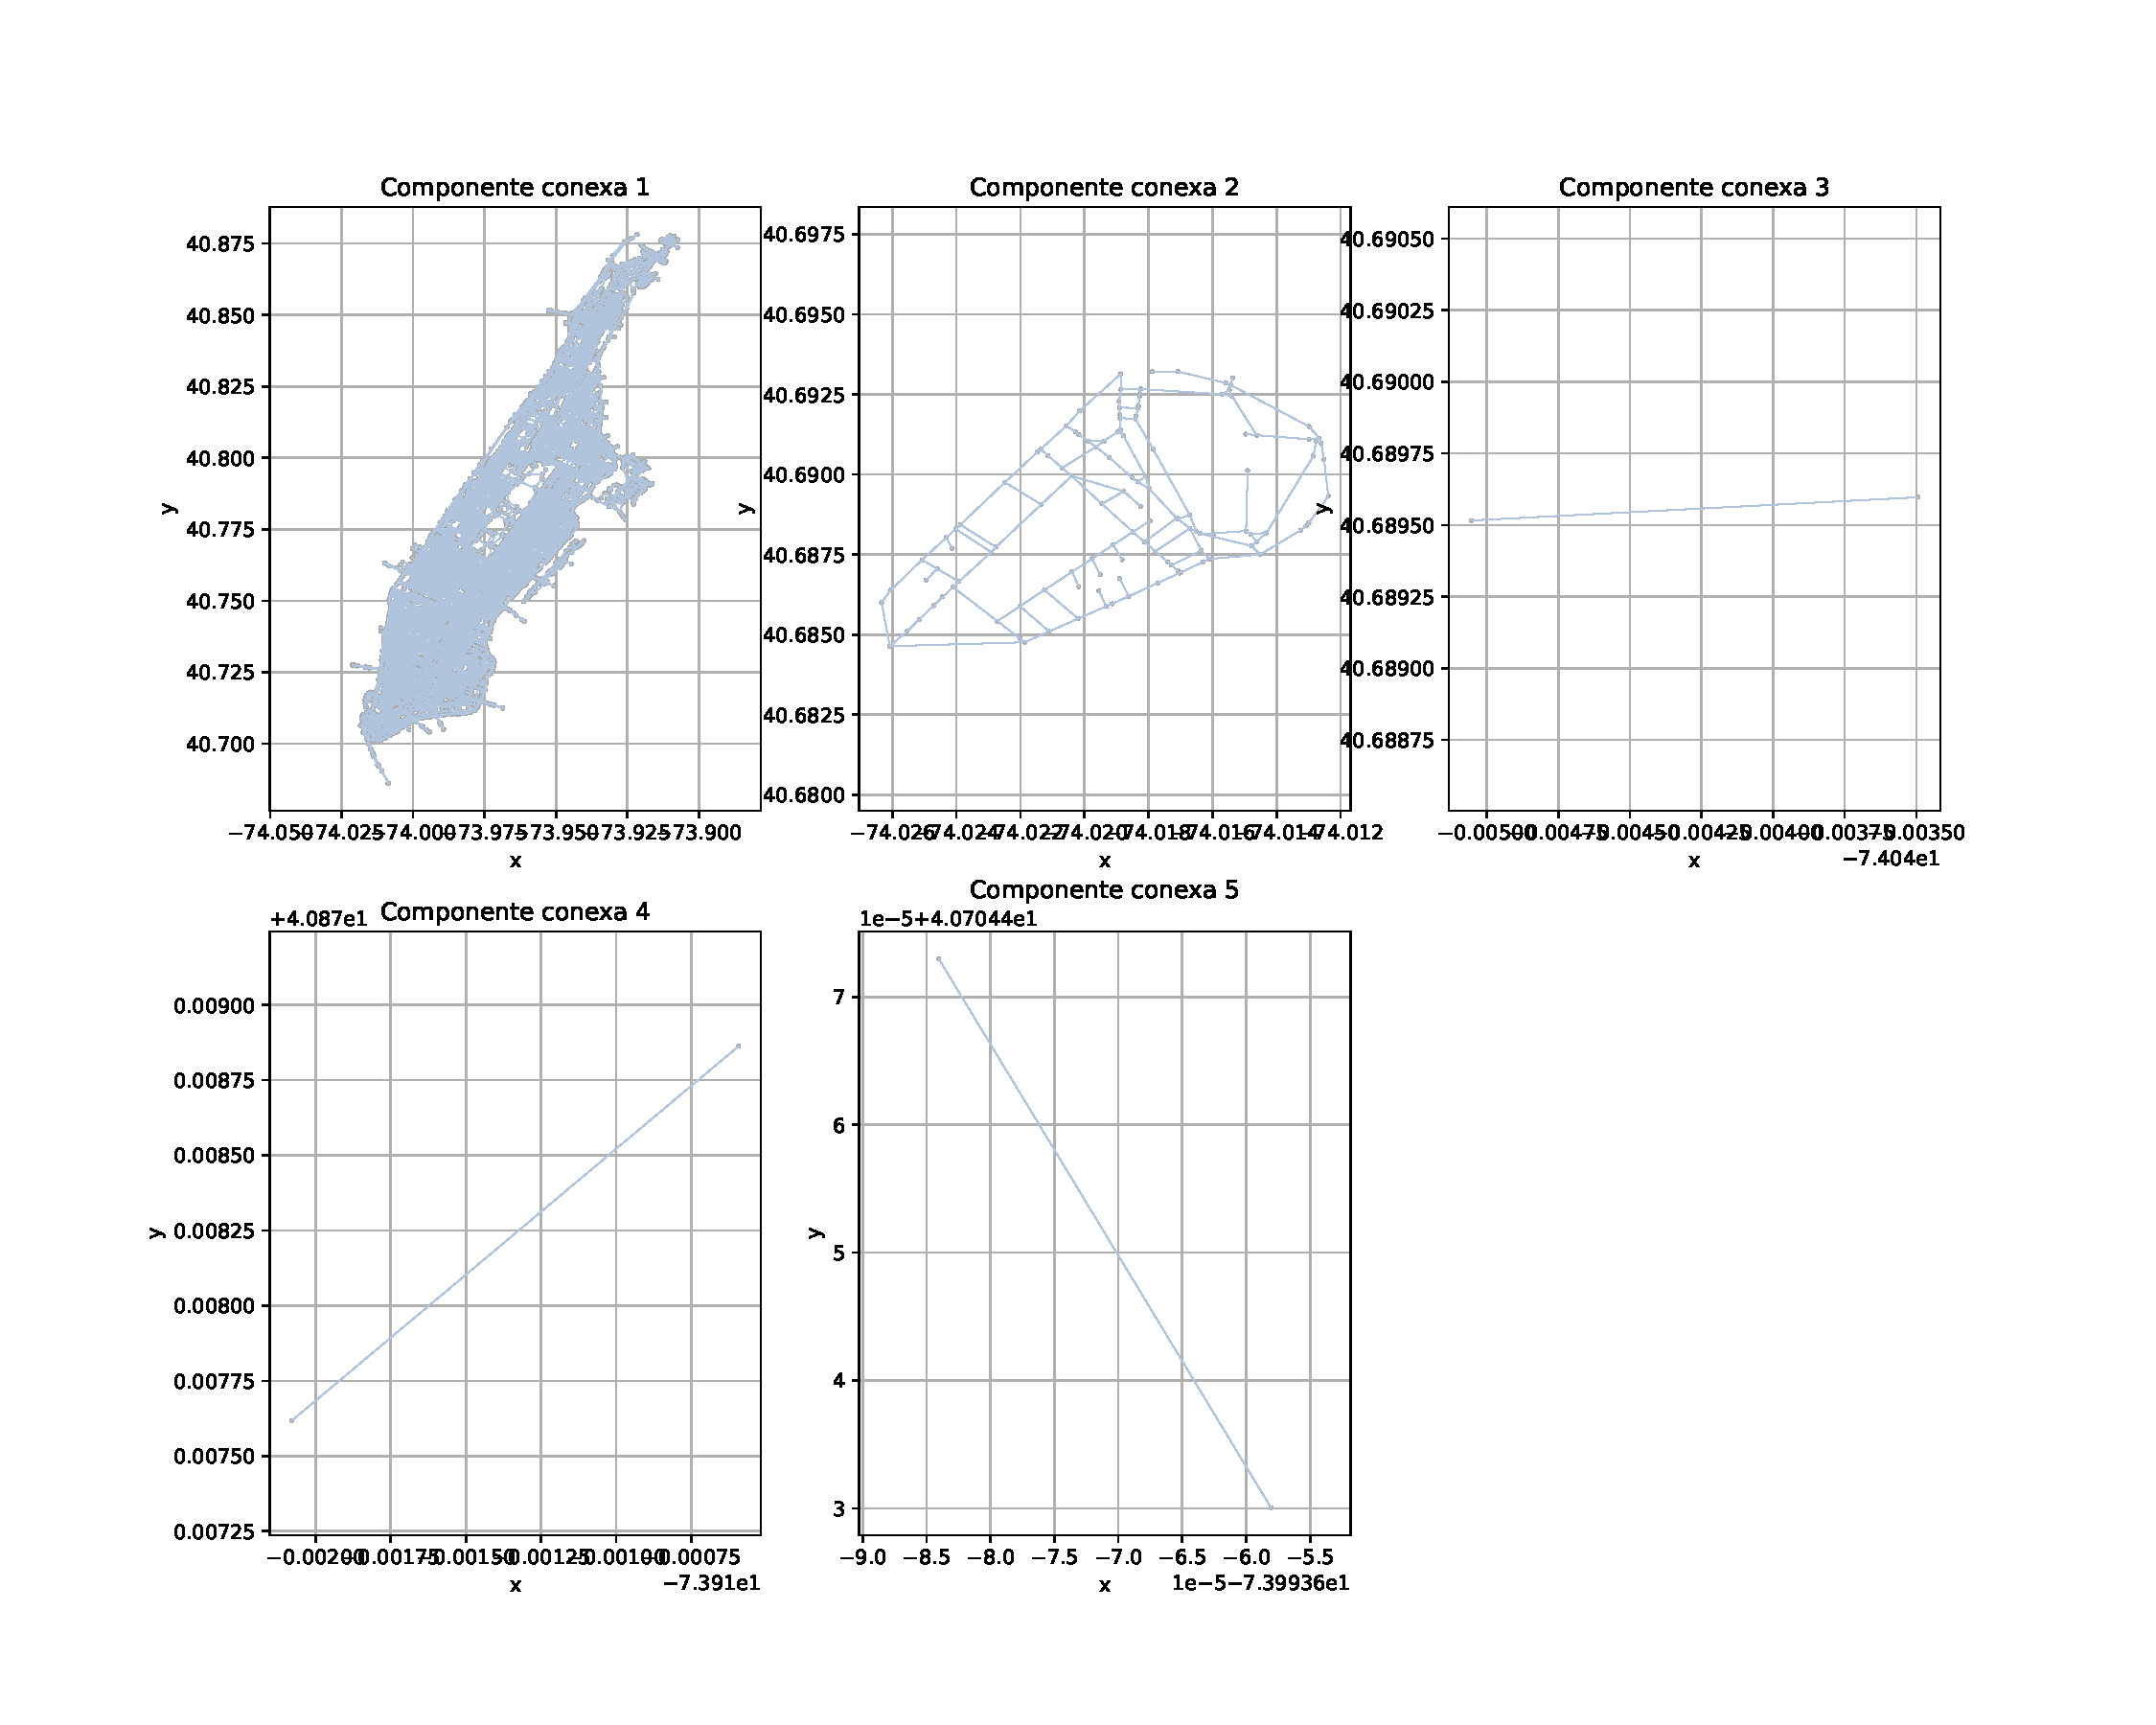
\includegraphics[width=0.7\textwidth, trim={5.4cm 2.3cm 5.4cm 3.7cm},clip]{../figs/fig2.pdf}
        
        Figura 2
    \end{figure}

    \vspace{2cm}

    \begin{figure}[ht]
        \centering
        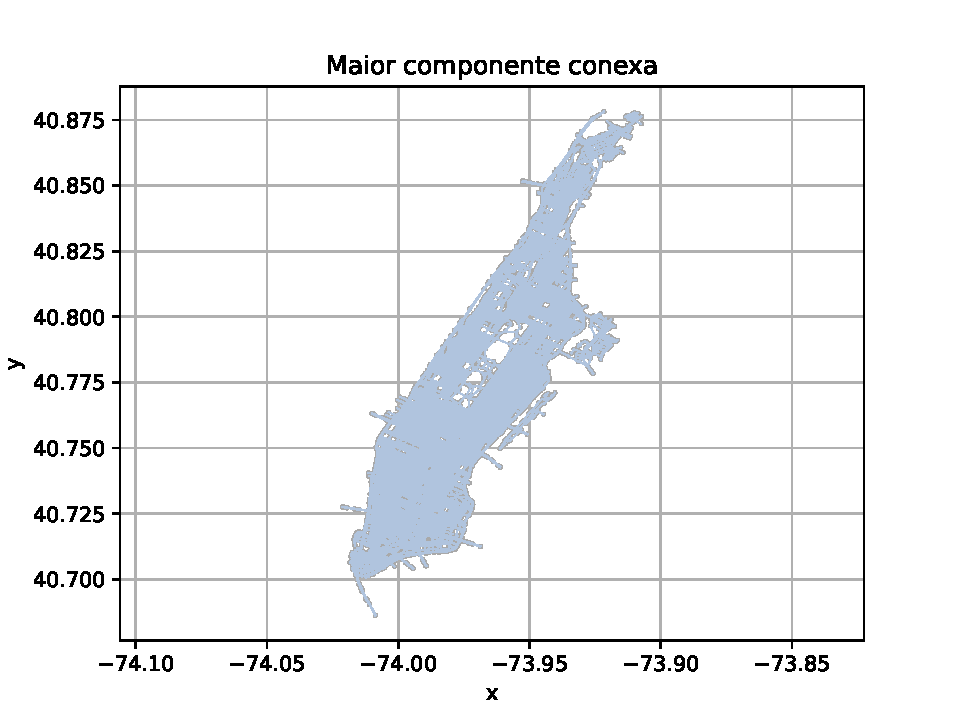
\includegraphics[width=0.7\textwidth, trim={5px 10px 15px 25px},clip]{../figs/fig3.pdf}
        
        Figura 3
    \end{figure}

    \newpage

    \phantom{}

    \vspace{3cm}

    \begin{figure}[ht]
        \centering
        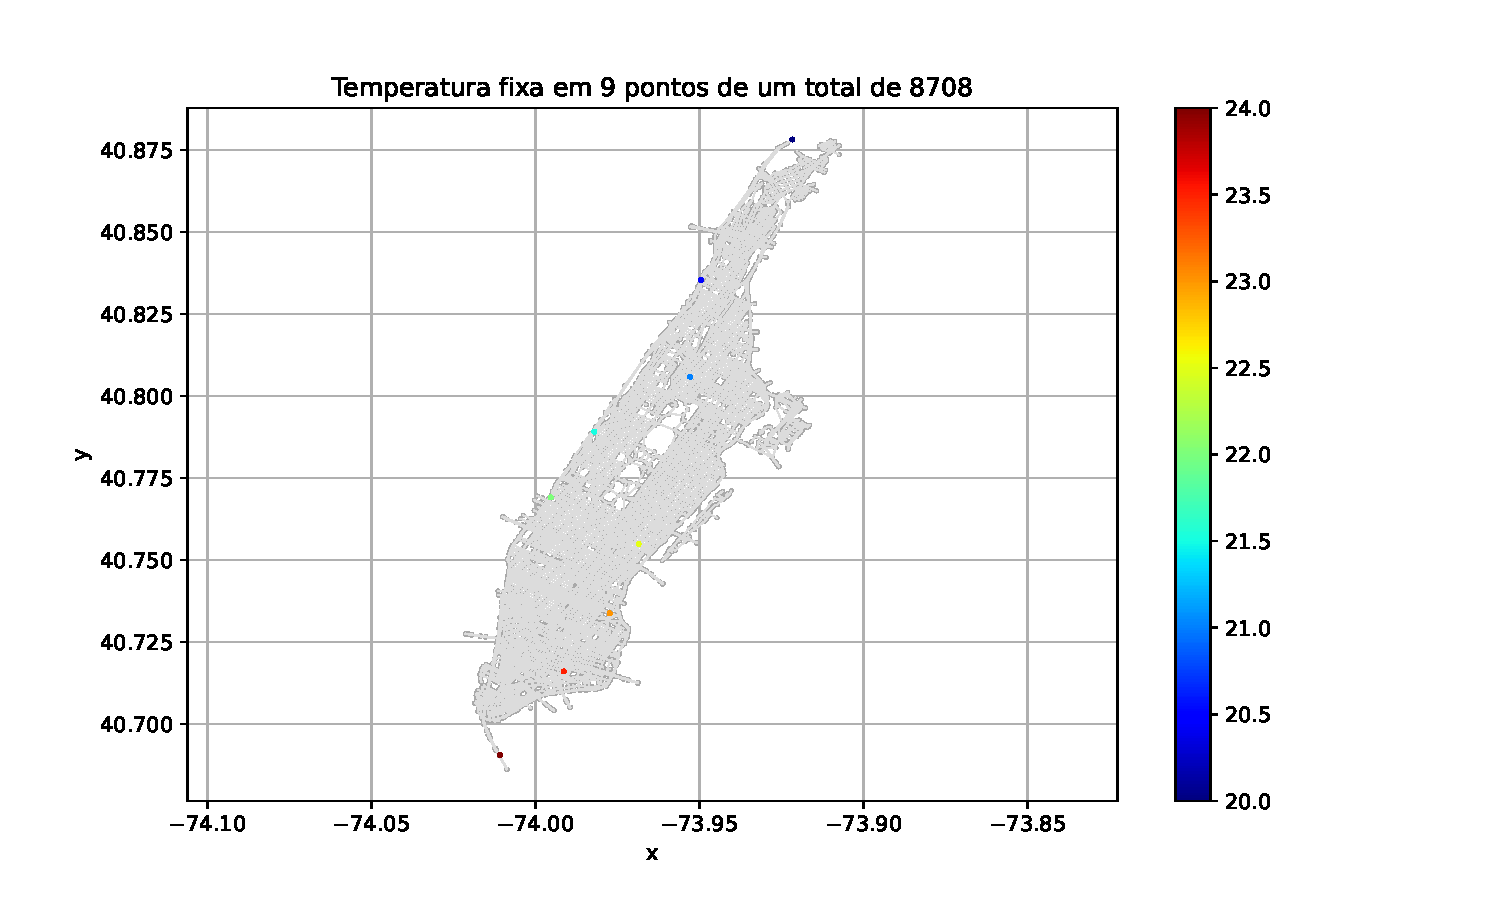
\includegraphics[width=1\textwidth, trim={5px 10px 55px 25px},clip]{../figs/fig4.pdf}
        
        \LARGE{Figura 4}
    \end{figure}

    \newpage

    \hypertarget{2}{}
    \begin{figure}[ht]
        \centering
        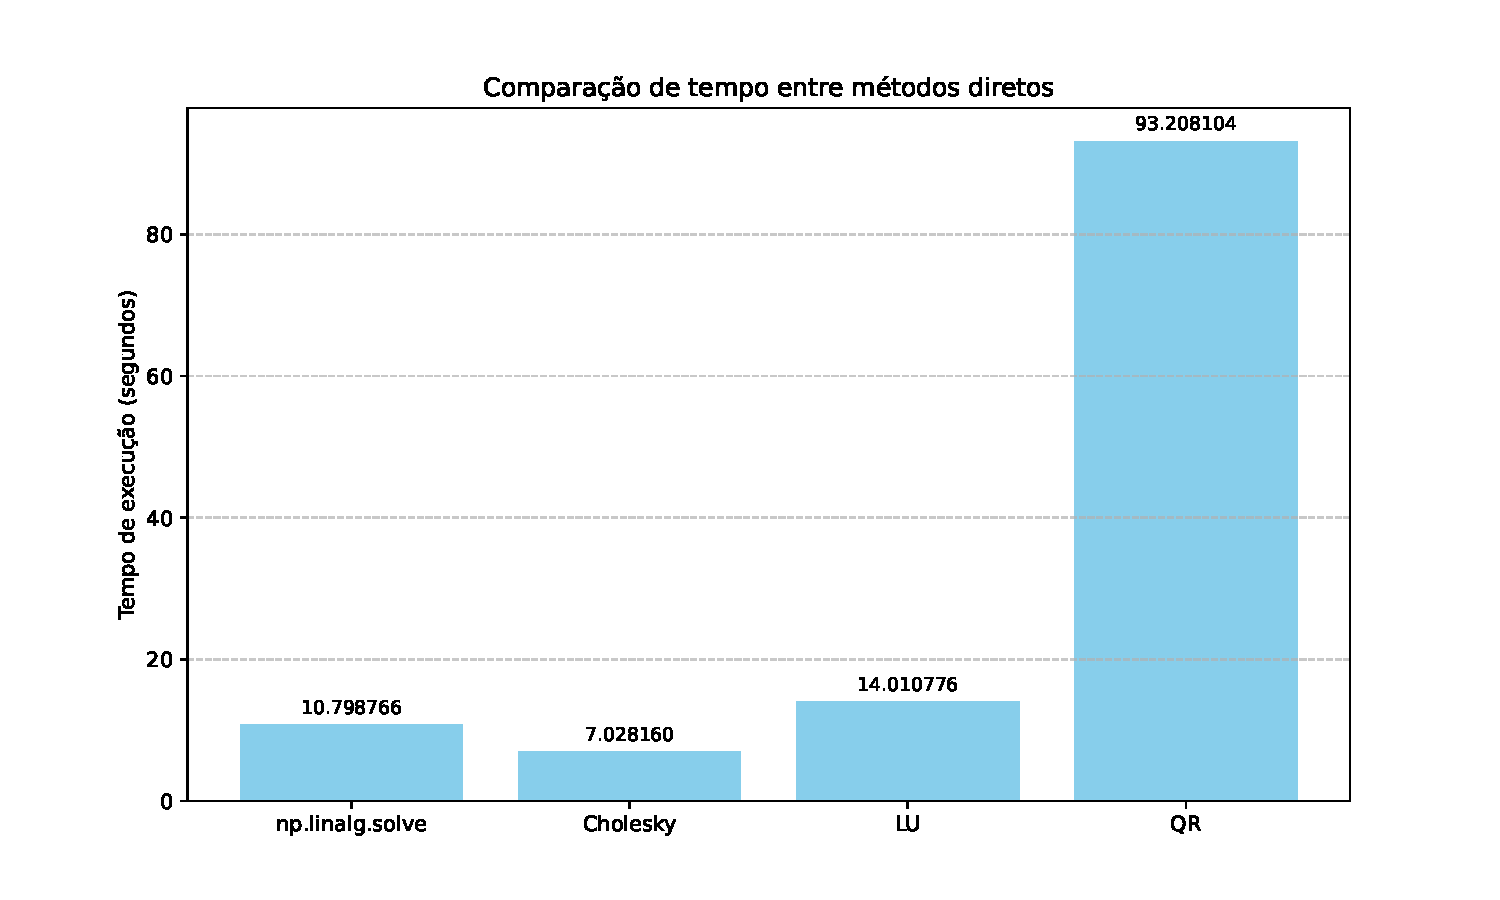
\includegraphics[width=0.8\textwidth, trim={5px 10px 15px 25px},clip]{../figs/fig5.pdf}
        
        \hyperlink{1}{Figura 5}
    \end{figure}

    \vspace{2cm}

    \hypertarget{4}{}
    \begin{figure}[ht]
        \centering
        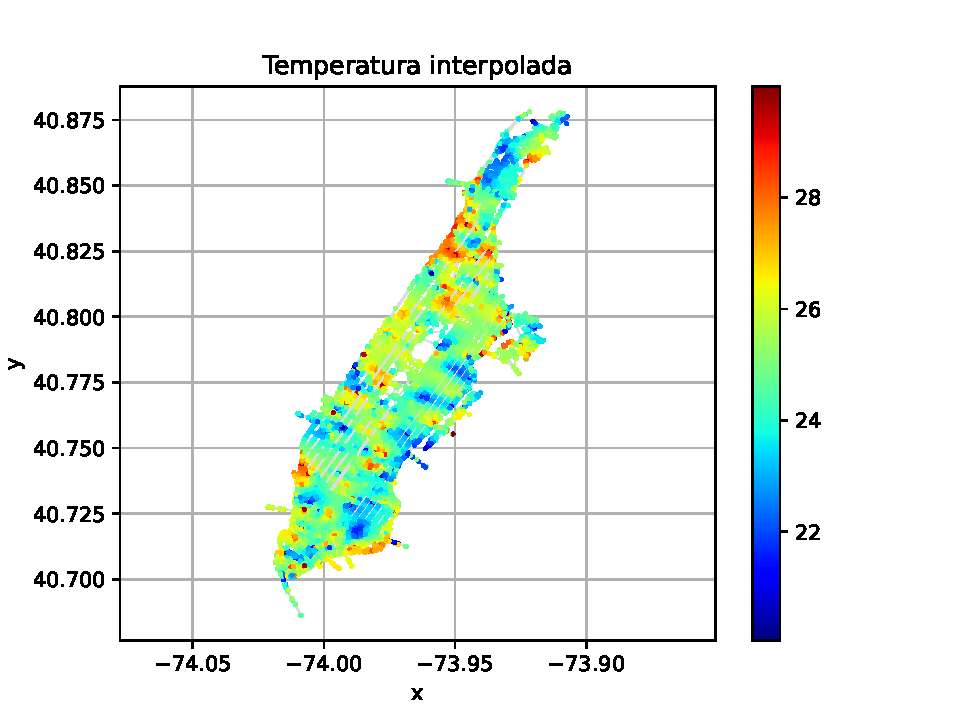
\includegraphics[width=0.8\textwidth, trim={5px 10px 15px 25px},clip]{../figs/fig6.pdf}
        
        \hyperlink{3}{Figura 6}
    \end{figure}

    \newpage

    \phantom{}

    \vspace{3cm}

    \begin{figure}[ht]
        \centering
        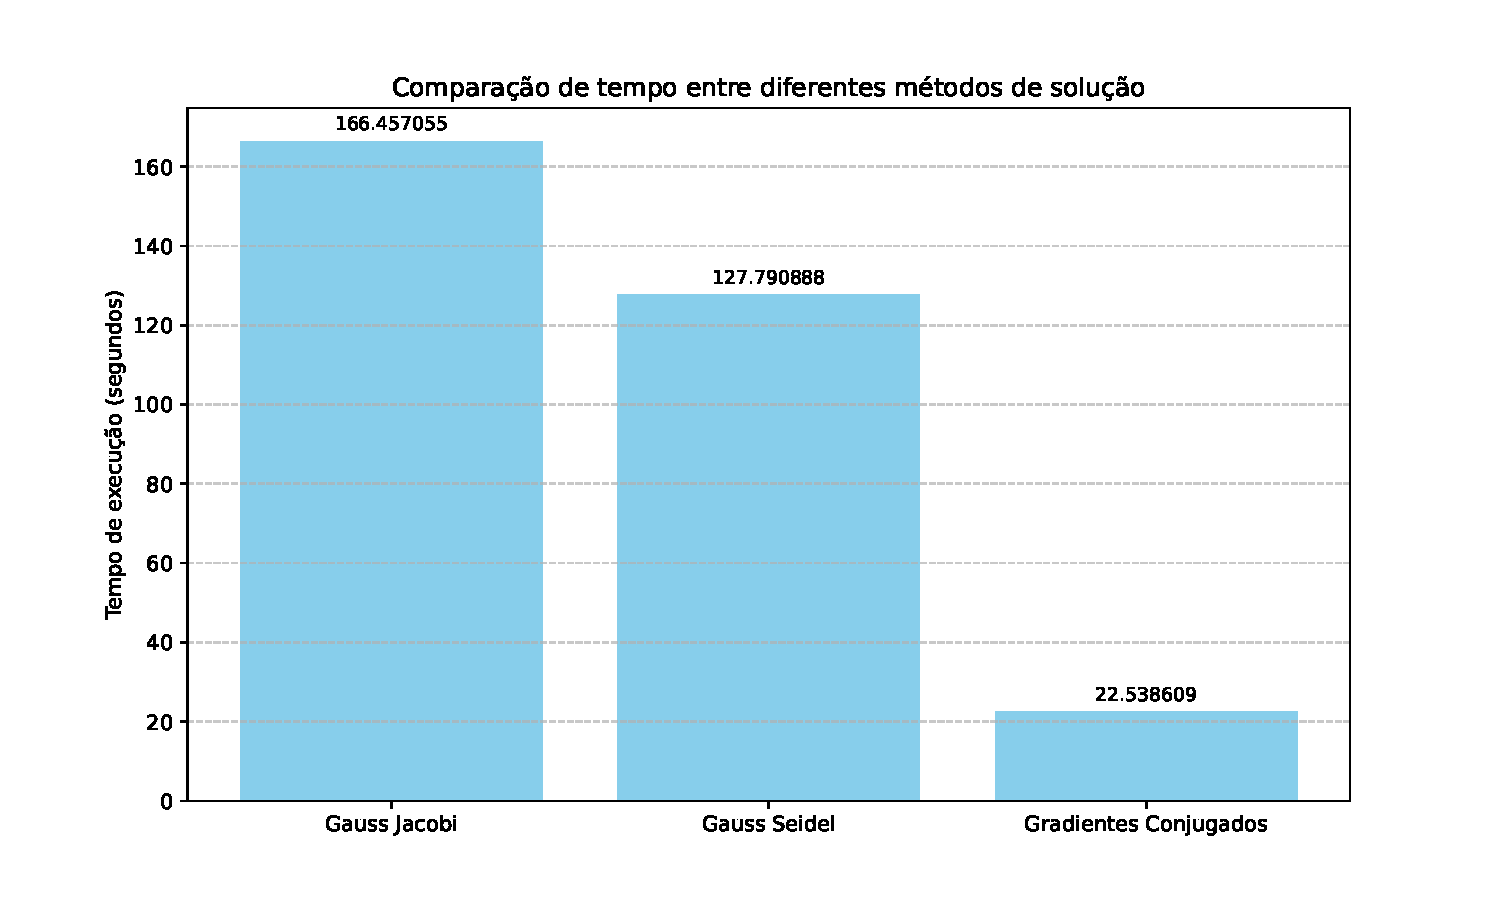
\includegraphics[width=1\textwidth, trim={5px 10px 55px 25px},clip]{../figs/fig7.pdf}
        
        \LARGE{Figura 7}
    \end{figure}

    \newpage

    \begin{figure}[ht]
        \centering
        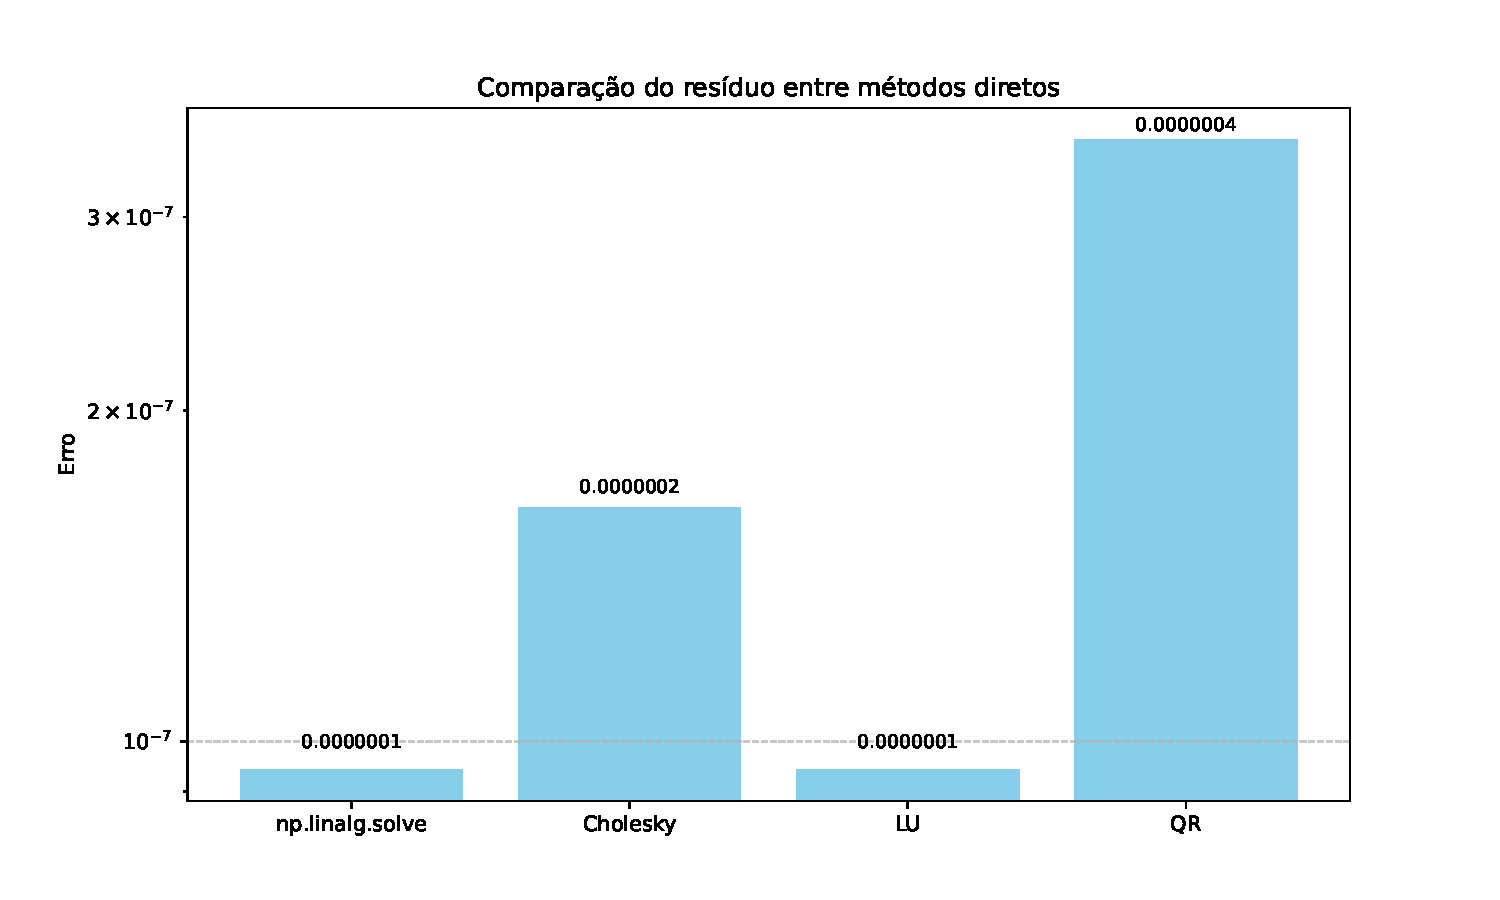
\includegraphics[width=0.8\textwidth, trim={5px 10px 15px 25px},clip]{../figs/fig8.pdf}
        
        Figura 8
    \end{figure}

    \vspace{2cm}

    \begin{figure}[ht]
        \centering
        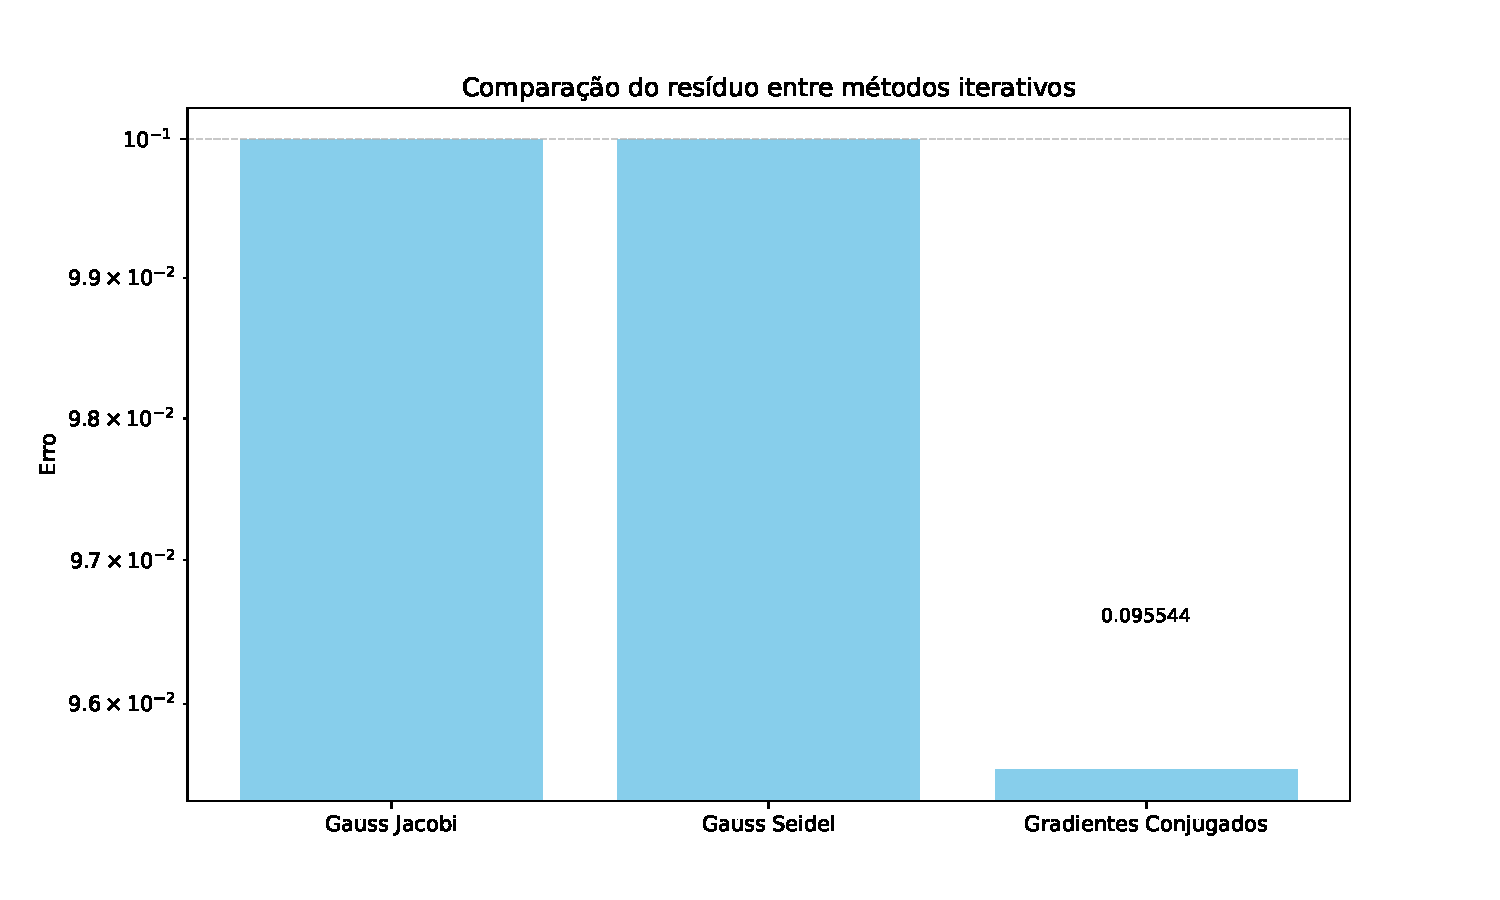
\includegraphics[width=0.8\textwidth, trim={5px 10px 15px 25px},clip]{../figs/fig9.pdf}
        
        Figura 9
    \end{figure}

    \newpage

    \phantom{}

    \vspace{3cm}

    \begin{figure}[ht]
        \centering
        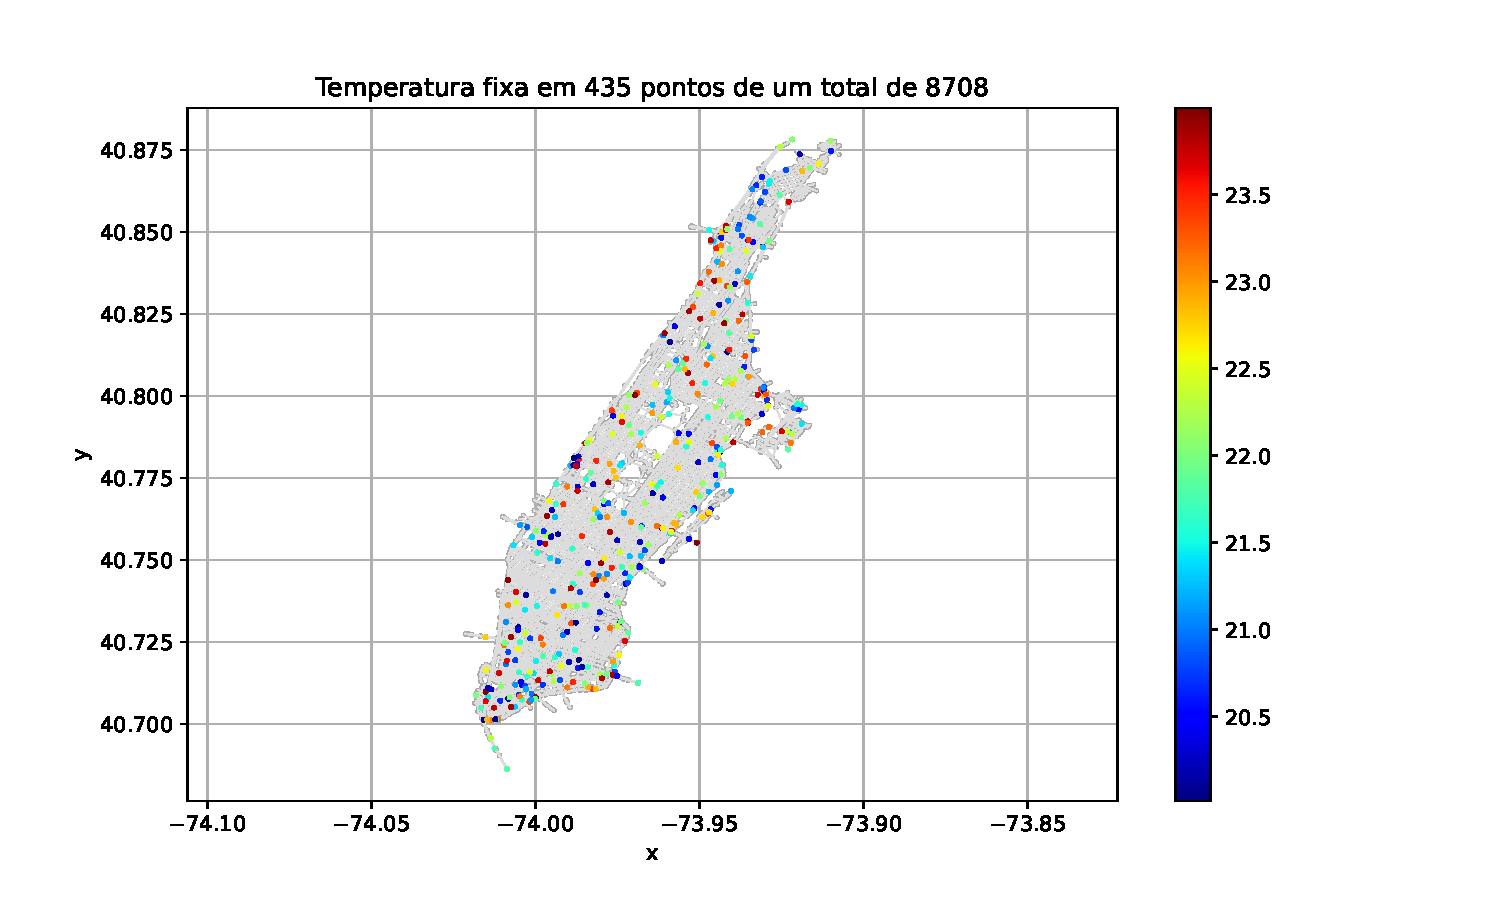
\includegraphics[width=1\textwidth, trim={5px 10px 55px 25px},clip]{../figs/fig10.pdf}
        
        \LARGE{Figura 10}
    \end{figure}

    \newpage

    \hypertarget{6}{}
    \begin{figure}[ht]
        \centering
        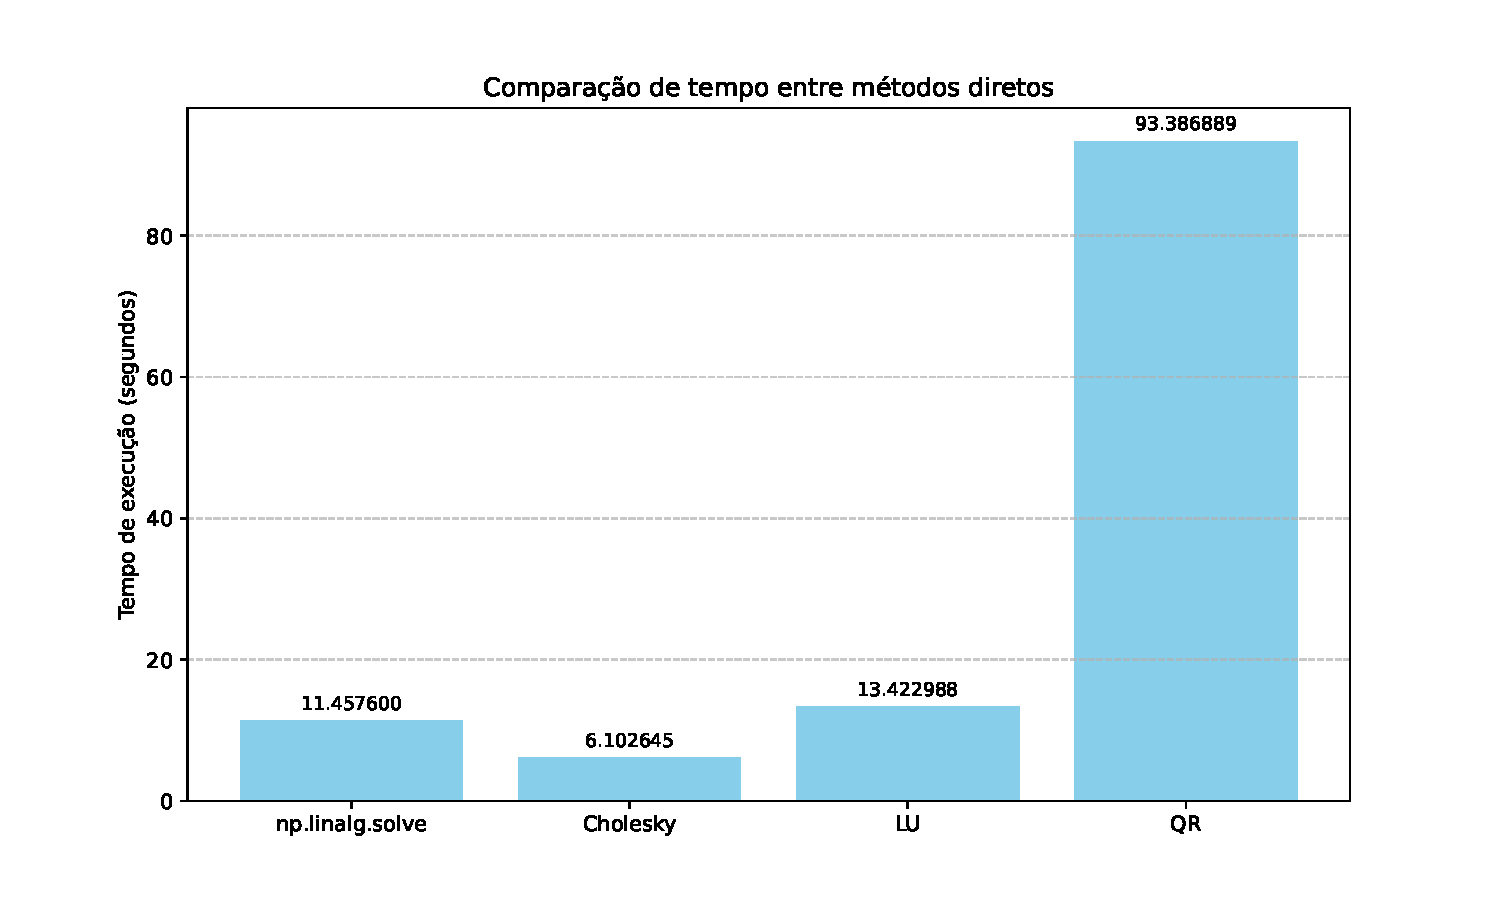
\includegraphics[width=0.8\textwidth, trim={5px 10px 15px 25px},clip]{../figs/fig11.pdf}
        
        \hyperlink{5}{Figura 11}
    \end{figure}

    \vspace{2cm}

    \hypertarget{8}{}
    \begin{figure}[ht]
        \centering
        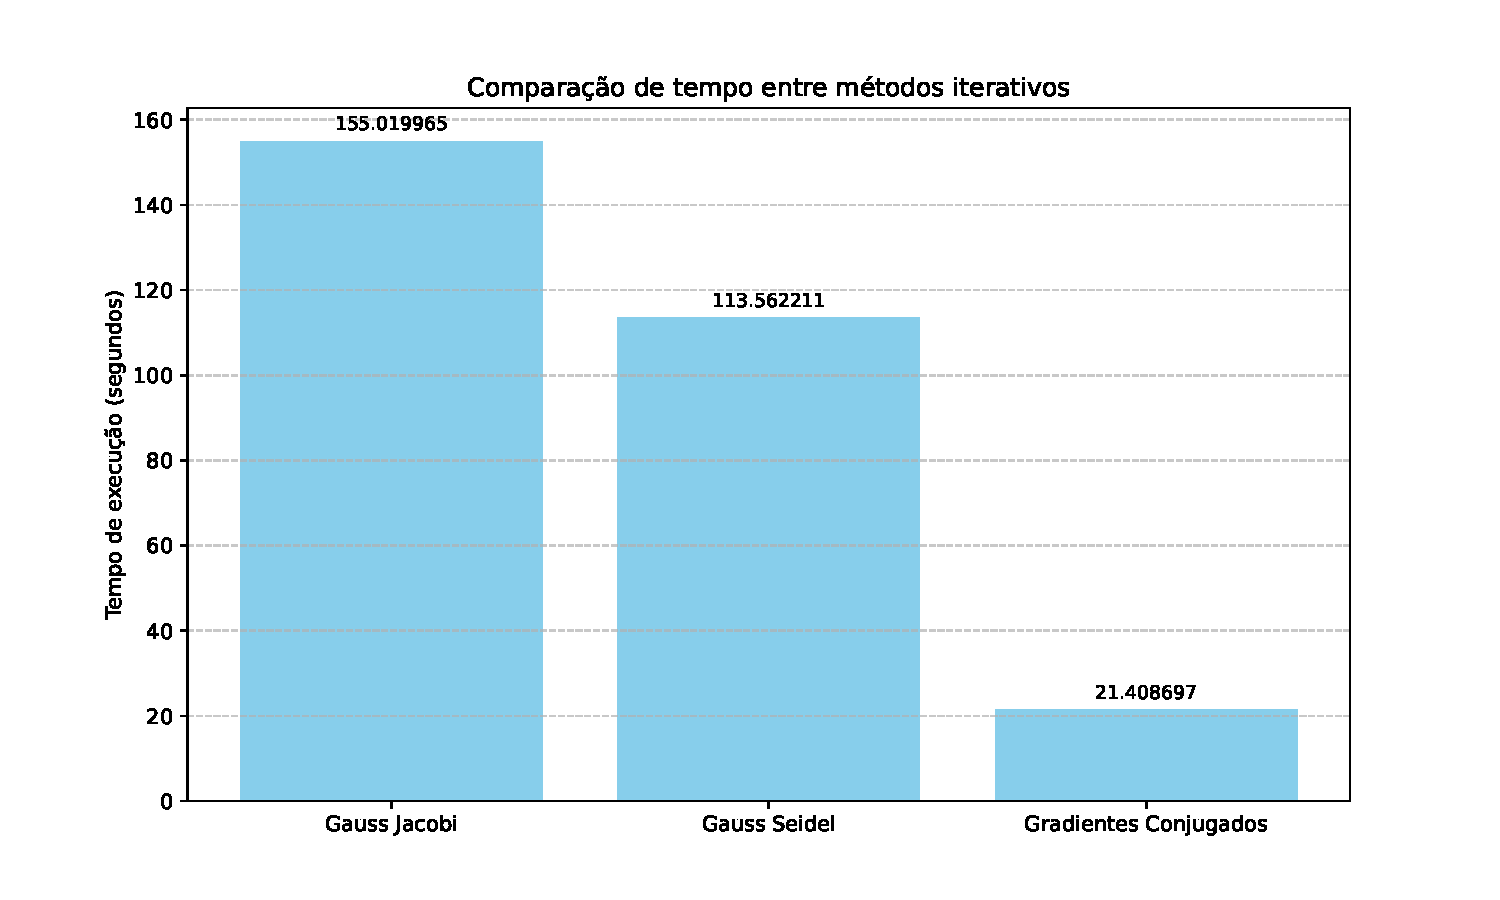
\includegraphics[width=0.8\textwidth, trim={5px 10px 15px 25px},clip]{../figs/fig12.pdf}
        
        \hyperlink{7}{Figura 12}
    \end{figure}

    \newpage

    \phantom{}

    \vspace{3cm}

    \begin{figure}[ht]
        \centering
        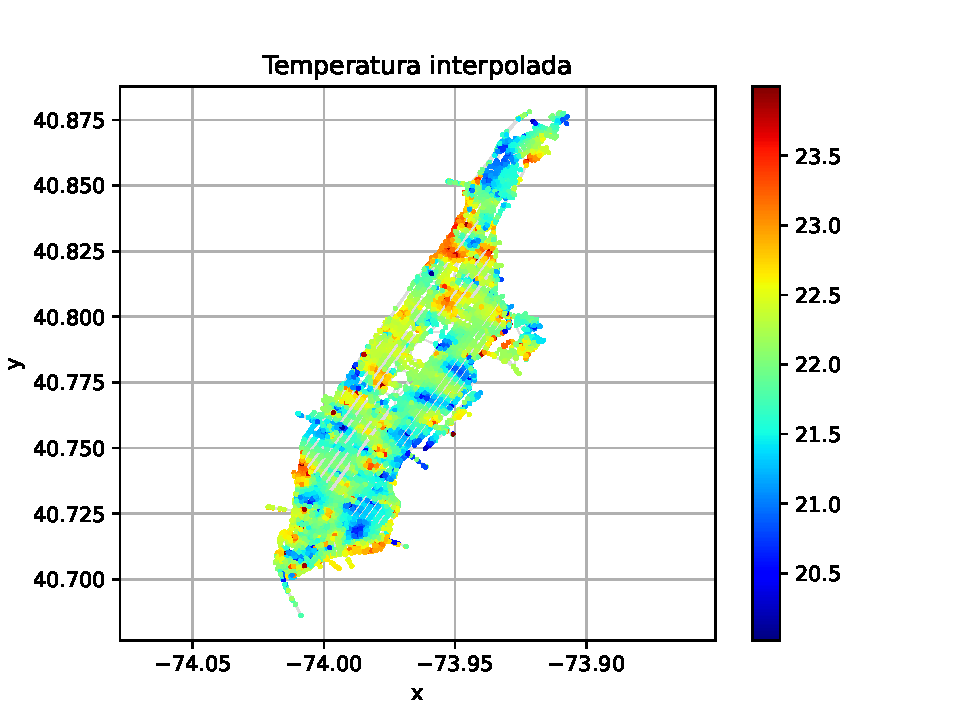
\includegraphics[width=1\textwidth, trim={5px 10px 55px 25px},clip]{../figs/fig13.pdf}
        
        \LARGE{Figura 13}
    \end{figure}

    \newpage

    \begin{figure}[ht]
        \centering
        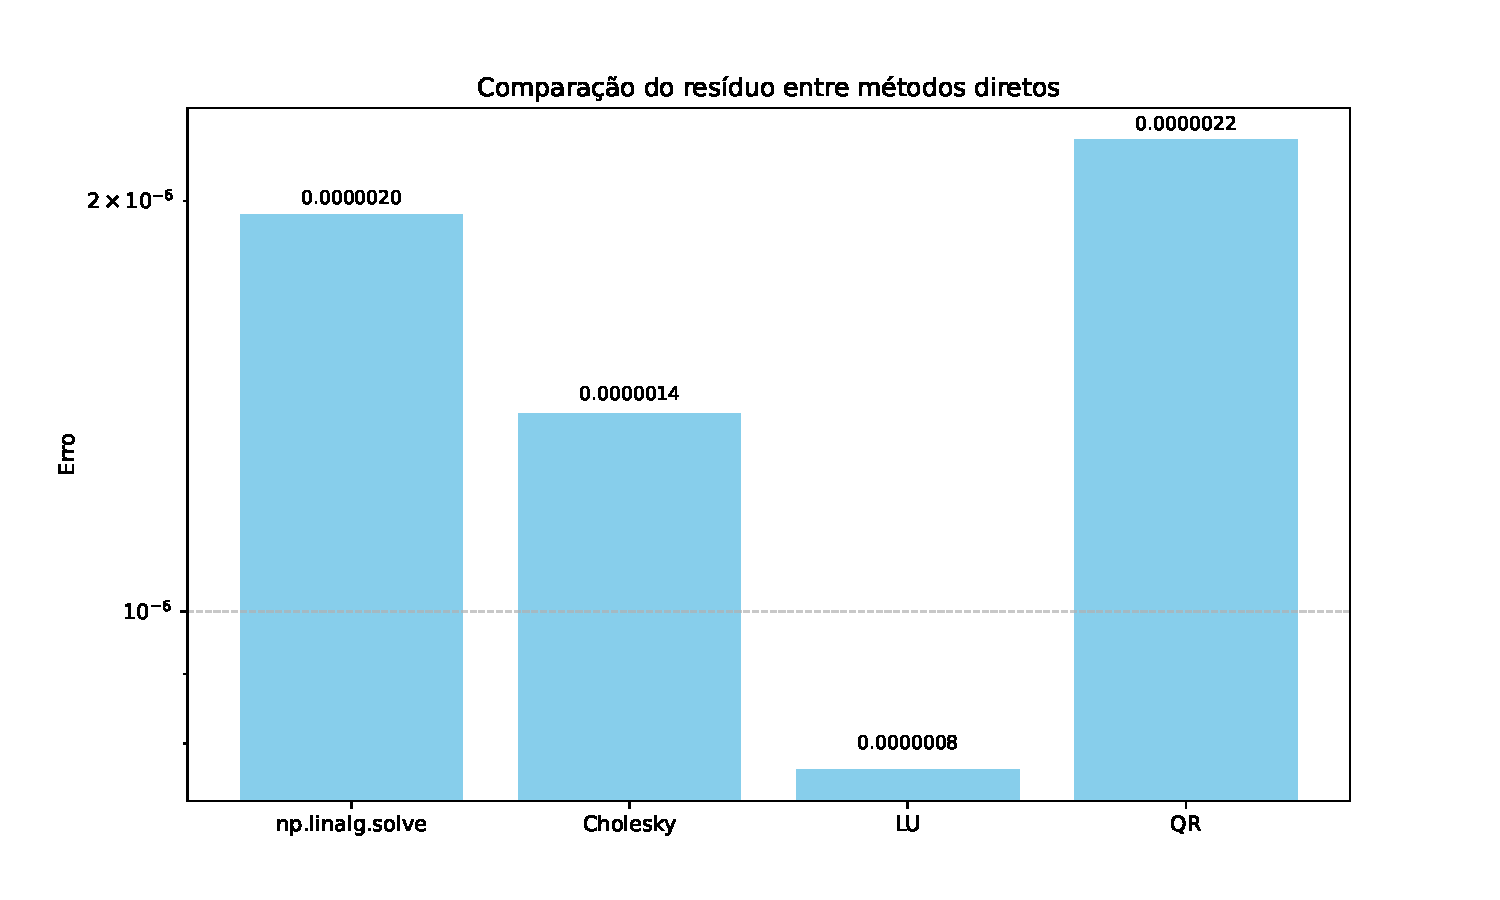
\includegraphics[width=0.7\textwidth, trim={5px 10px 15px 25px},clip]{../figs/fig14.pdf}
        
        Figura 14
    \end{figure}

    \vspace{2cm}

    \begin{figure}[ht]
        \centering
        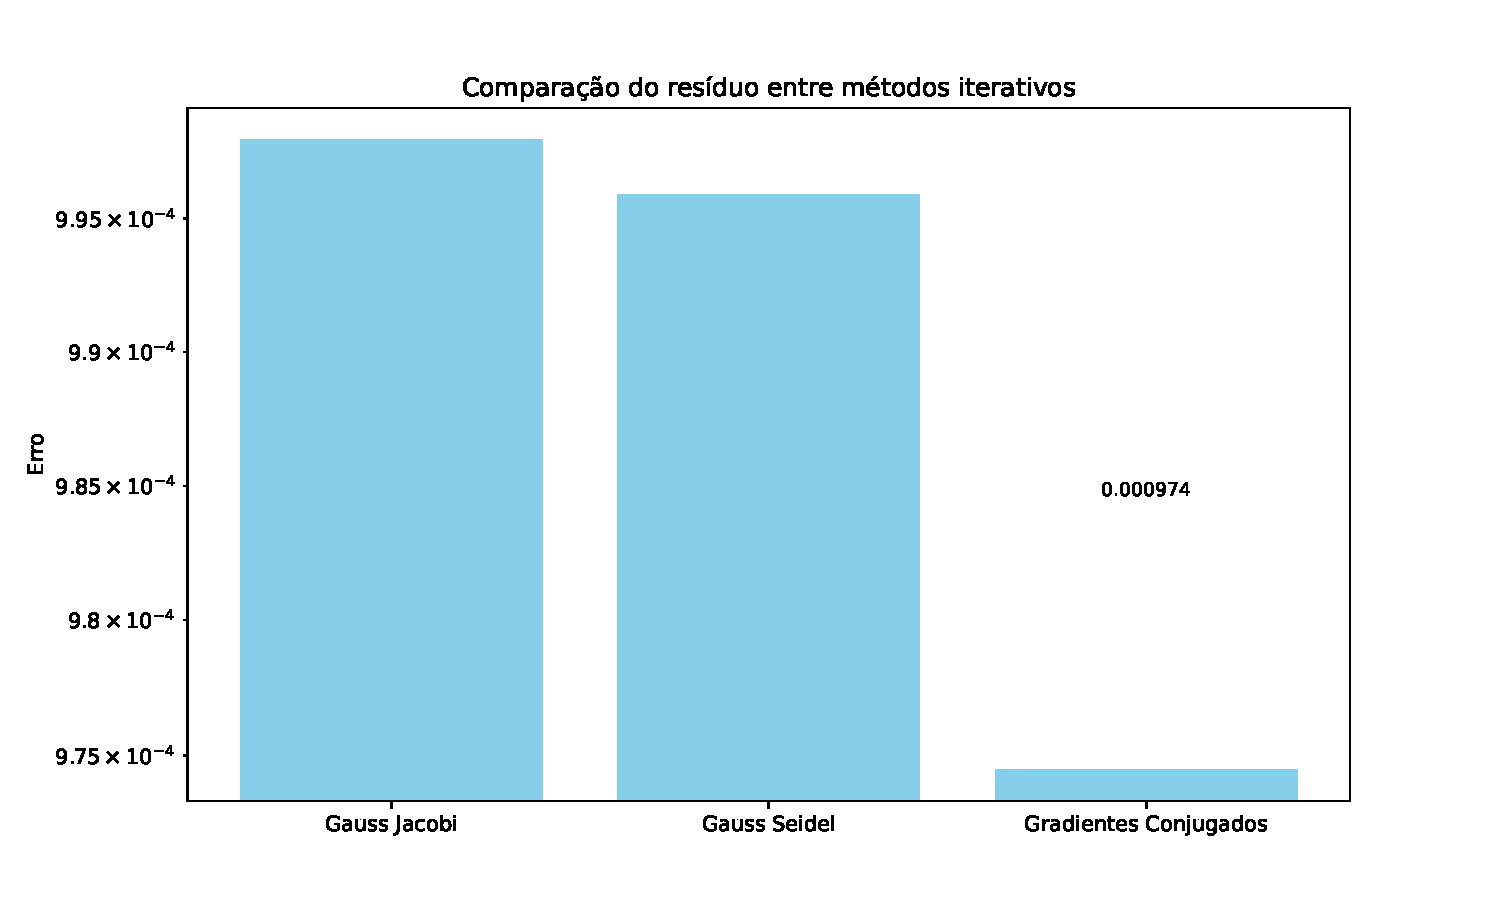
\includegraphics[width=0.7\textwidth, trim={5px 10px 15px 25px},clip]{../figs/fig15.pdf}
        
        Figura 15
    \end{figure}
\end{document}